\documentclass[Bachelorarbeit.tex]{subfiles}
\begin{document}

\graphicspath{{./figures/newMarket/}}	%specifying the folder for the figures

\chapter{A new Market}
As already introduced in chapter \ref{ch:interpretation} "Interpretation" a new market is necessary to repair the miss-allocation of collateralized assets in the range of the pessimist agents by enabling the agents to trade collateralized assets against cash.

\section{Implementation}

\subsection{Price-Range}
As for all other 3 Markets the price-ranges of the offers must be defined. Note that all prices must obviously be in the unit of cash.

\paragraph{minimum}
When calculating the minimum price of a collateralized asset - that is how much is the collateralized asset minimally worth - it is important to include the collateral-aspect of the asset. Thus one starts with the minimum asset-price in cash which is the down-price \textit{pD} and subtracts the maximum possible amount of cash which is bound through a bond as collateral which is the face-value \textit{V}. This value is a constant for all agents.

\begin{center}
$\textit{min collateralized asset-price} = \min(0, \textit{pD} - \textit{V})$
\end{center}
 
\paragraph{maximum}
To calculate the maximum price of a collateralized asset - that is how much is the collateralized asset maximally worth - one needs to include the collateral-aspect of the asset too. Equal to calculating the minimum one starts now with the maximum asset-price in cash which is the up-price \textit{pU} and subtracts the minimum possible amount of cash which is bound through a bond as collateral which is the face-value \textit{pD}. This value is a constant for all agents.

\begin{center}
$\textit{max collateralized asset-price} = \textit{pU} - \textit{pD}$
\end{center}

\paragraph{limit}
Applying the same rules as in minimum and maximum to the limit price calculation one needs to subract the limit-price of loans from the limit-price of asset to receive the limit-price of a collateralized asset. This value is individual for each agent as the limit-prices differ across the agents both for assets and loans.

\begin{center}
$\textit{limit-price of collateralized asset} = \textit{limit-price of asset} - \textit{limit-price of loan}$
\end{center}

\subsection{Bid-Offering}
The way bid-offers are generated is very similar to the "Bond against Cash" market. Bid Offerings are generated only when the agent has any cash holdings. The price is drawn randomly between the minimum price and the limit-price because when buying one wants to buy below the expected value to make a profit. As amount one TRADING-UNIT of an asset is selected - in the thesis-implementation 0.1 - but if there is not enough cash left to buy one TRADING-UNIT of assets then the amount of assets is selected which can be bought with the remaining cash holdings.

\begin{table}[h]
	\centering
	\caption{Bid-Offering parameters}
	\begin{tabular} { l c r }
		\hline
		Pre-Condition & $\textit{cash holdings} > 0$  \\
		Asset-Price & $\mathrm{random}(\textit{min coll. asset-price}, \textit{limit-price of coll. asset})$ \\
		Asset-Amount & $\min ( \frac{ \textit{cash holdings} }{ \textit{Asset-Price} }, \textit{TRADING-UNIT} )$ \\
		\hline
	\end{tabular}
\end{table}


\subsection{Ask-Offering}
The way ask-offers are generated is very similar to the "Bond against Cash" market. Ask Offerings are generated only when the agent has any collateralized assets. The price is drawn randomly between the limit-price and maximum price because when selling one wants to sell above the expected value to make a profit. As amount one TRADING-UNIT of an asset is selected - in the thesis-implementation 0.1 - but if there are fewer collateralized assets left then the remaining amount of collateral is selected.

See Chapter \ref{ch:implementation} "Implementation" for the equation of collateral holdings.

\begin{table}[h]
	\centering
	\caption{Ask-Offering parameters}
	\begin{tabular} { l c r }
		\hline
		Pre-Condition & $\textit{collateral holdings} > 0$  \\
		Asset-Price & $\mathrm{random}(\textit{limit-price of coll. asset}, \textit{max coll. asset-price})$ \\
		Asset-Amount & $\min ( { \textit{collateral holdings} }, \textit{TRADING-UNIT} )$ \\
		\hline
	\end{tabular}
\end{table}

\subsection{Match}
Below the wealth-exchange table is given in case of a match between two agents on the new market.

\begin{table}[h]
	\centering
	\caption{Wealth-Exchange on match}
	\begin{tabular} { l c r }
		& Seller & Buyer \\
		\hline
		Loan Given & + matching-amount & N/A \\
		Loans Taken & N/A & - matching-amount \\
		Assets holdings & - matching-amount & + matching-amount \\
		Cash holdings  & + matching-price & - matching-price \\
		\hline
	\end{tabular}
\end{table}

\section{Results}
Of most importance are the results of the simulation when using the new market. The plain results are given in this section where the interpretation of the results are given in the following section.

\medskip

As experiment-configuration the same is used as given in Chapter \ref{ch:results} "Results" except that the new market is now included in the simulation too.

\subsection{Fully-Connected topology}
\begin{table}[h]
	\centering
	\caption{Configuration for all experiments}
	\begin{tabular} { l c r }
		\hline
		Agent-Count & 100 \\
		Bond-Type & 0.5 \\
		Replication-Count & 50 \\
		Terminate after & 1000 failed successive Transactions \\
		\hline
	\end{tabular}
\end{table}

\begin{figure}[H]
	\centering
  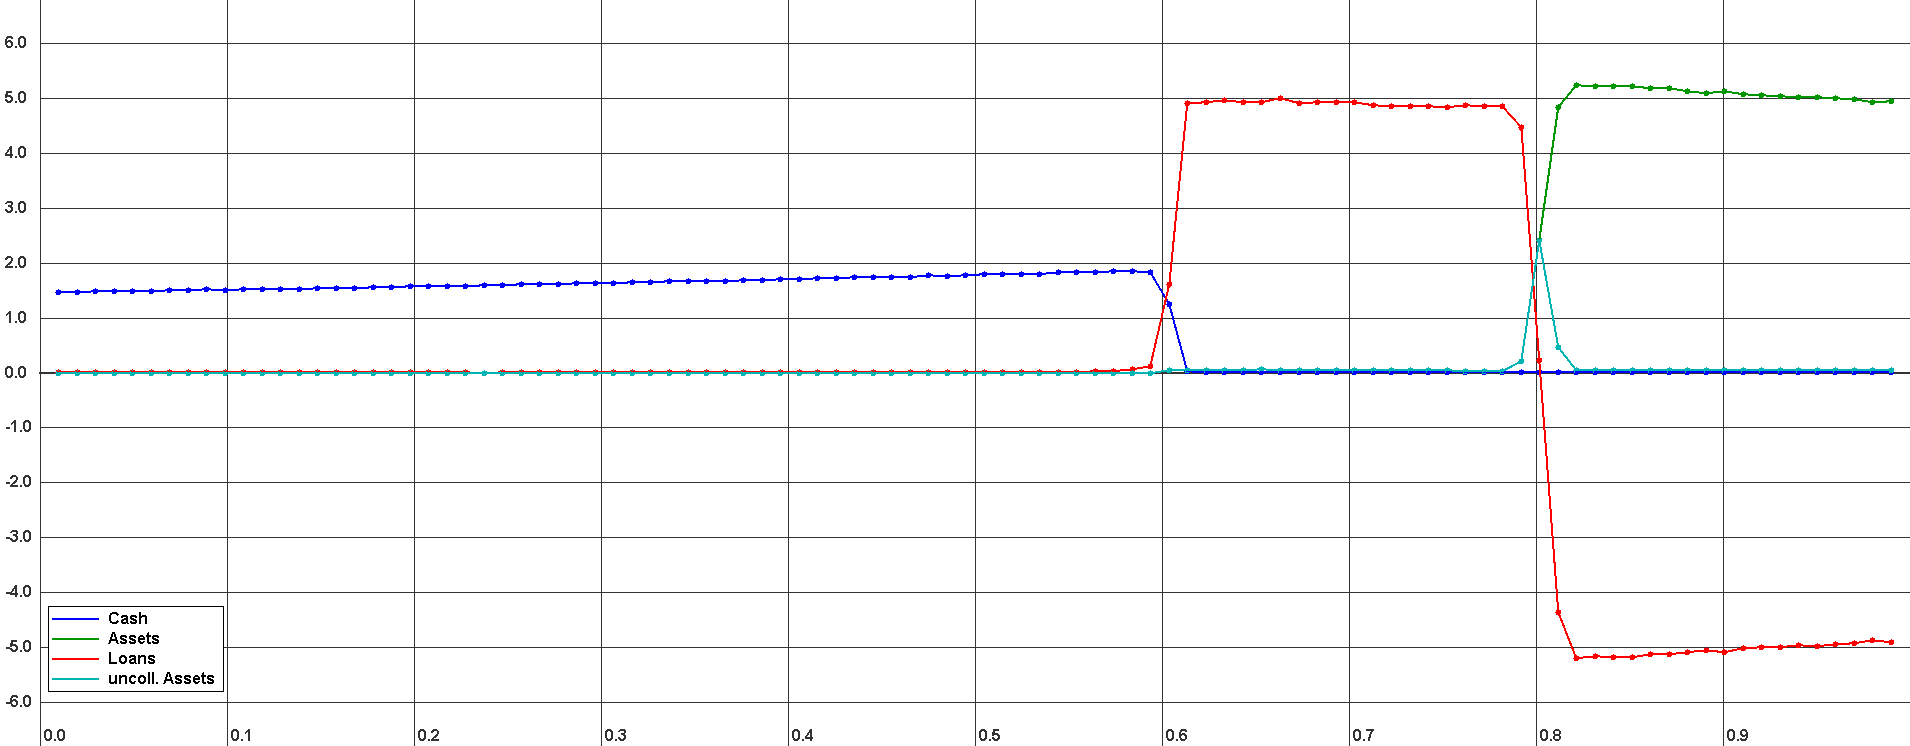
\includegraphics[width=1.0\textwidth, angle=0]{FULLYCONNECTED_100_WITHCOLLATERALMARKET_REPL.png}
	\caption{Wealth-Distribution of Fully-Connected topology with collateral/cash market}
	\label{fig:wealth_FULLYCONNECTED_100_WITHCOLLATERALMARKET_REPL}
\end{figure}

\begin{table}[h]
	\caption{Equilibrium of Fully-Connected topology with collateral/cash market}
	\centering
	\begin{tabular} { l c r }
		\hline
		Asset-Price & 0.688 (0.008) \\
		Loan-Price & 0.381 (0.002) \\
		Marginal Buyer i0 & 0.597 (0.005) \\
		Marginal Seller i1 & 0.803 (0.003) \\
		\hline
		Pessimist Wealth & 1.597 (0.009) \\
		Medianist Wealth & 4.76 (0.1) \\
		Optimist Wealth & 4.963 (0.052) \\
		\hline
	\end{tabular}
\end{table} 

\begin{table}[h]
	\caption{Performance of Fully-Connected topology with collateral/cash market}
	\centering
	\begin{tabular} { l c r }
		\hline
		Successful TX & 1916.14 (31.42) \\
		Total TX & 6364.8 (1679.21) \\
		Failed TX & 4448.66 (1668.93) \\
		\hline
	\end{tabular}
\end{table}

TODO: irgendeine statistischer test, der anhand mittelwert und standardabweichung vergleichen lässt?
T-Test?

\begin{table}[h]
	\caption{Difference to theoretical equilibrium as given in Table \ref{tab:theoretical_equilibrium_100Agents_05Bond} of Chapter \ref{ch:results} "Results"}
	\centering
	\begin{tabular} { l c c c r }
		& Value & Reference & difference to Reference \\
		\hline
		Asset-Price & 0.688 & 0.717 & -4.0\% \\
		Loan-Price & 0.381 & 0.375 & +1.6\% \\
		Marginal Buyer i0 & 0.597 & 0.584 & +2.2\% \\
		Marginal Seller i1 & 0.802 & 0.803 & +0.1\% \\
		\hline
	\end{tabular}
\end{table} 

\begin{table}[h]
	\caption{Difference to equilibrium without collateral/cash market as given in Table \ref{tab:fullyconnected_equilibrium_100Agents_05Bond} of Chapter \ref{ch:results} "Results"}
	\centering
	\begin{tabular} { l c c c r }
		& Value & Reference & difference to Reference \\
		\hline
		Asset-Price & 0.688 & 0.689 & -0.1\% \\
		Loan-Price & 0.381 & 0.384 & -0.7\% \\
		Marginal Buyer i0 & 0.597 & -0.006 & -1.0\% \\
		Marginal Seller i1 & 0.803 & 0.803 & 0.0\% \\
		\hline
		Pessimist Wealth & 1.597 & 1.597 & 0.0\% \\
		Medianist Wealth & 4.76 & 4.565 & +4.2\% \\
		Optimist Wealth & 4.963 & 5.02 & -1.1\% \\
		\hline
	\end{tabular}
\end{table} 


\subsection{Ascending-Connected topology}
\begin{figure}[H]
	\centering
  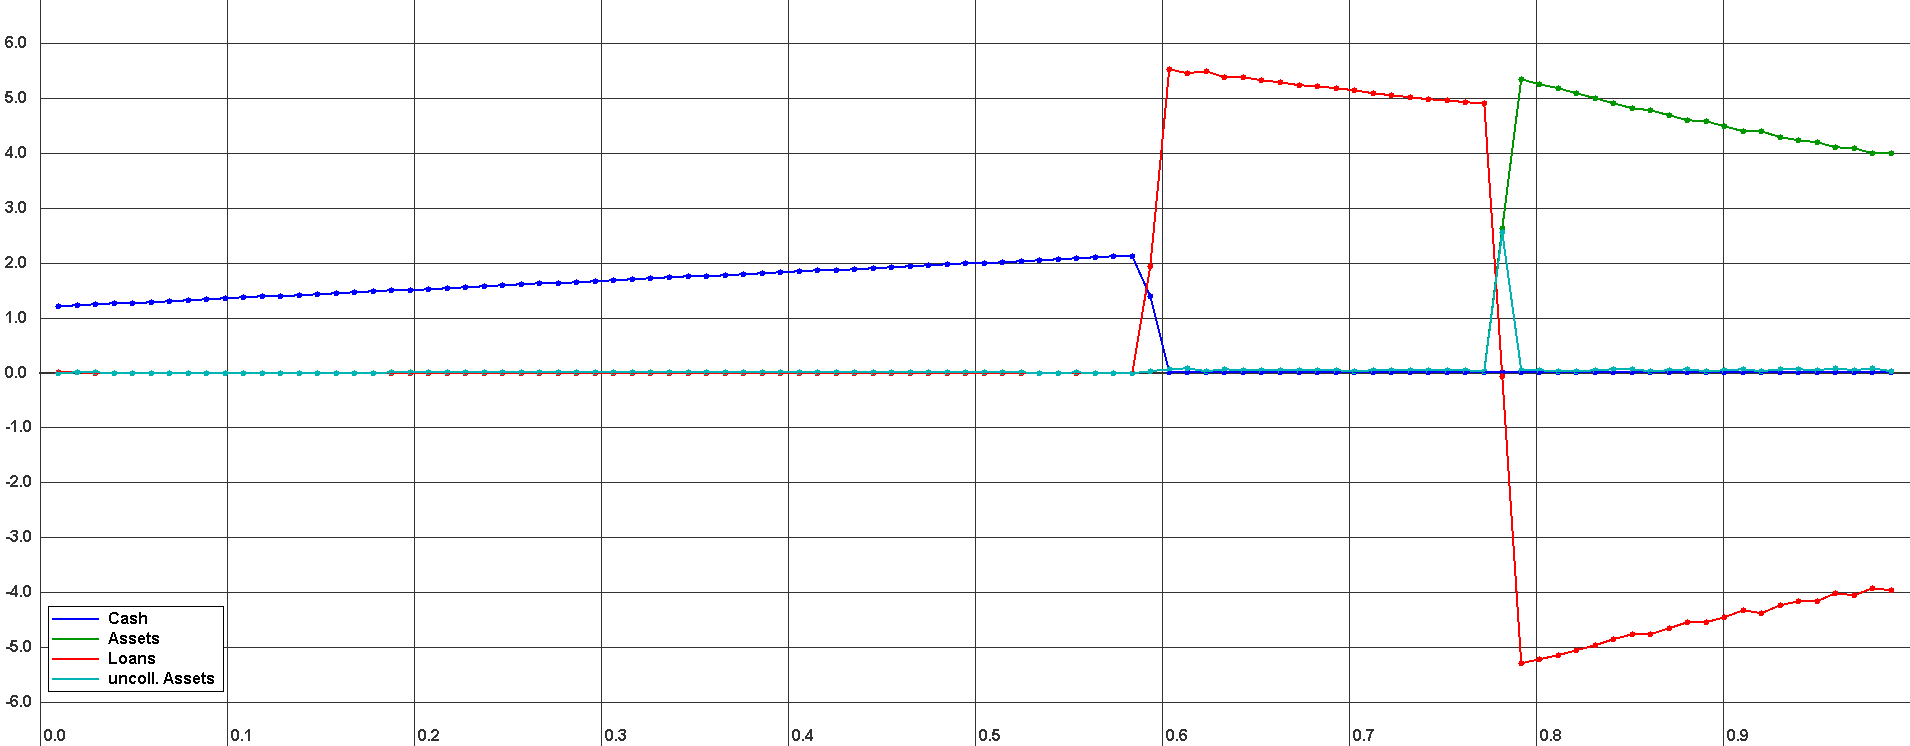
\includegraphics[width=1.0\textwidth, angle=0]{ASCENDINGCONNECTED_100_WITHCOLLATERALMARKET_REPL.png}
	\caption{Wealth-Distribution of Ascending-Connected topology with collateral/cash market}
	\label{fig:wealth_ASCENDINGCONNECTED_100_WITHCOLLATERALMARKET_REPL}
\end{figure}

\begin{table}[h]
	\caption{Equilibrium of Ascending-Connected topology}
	\centering
	\begin{tabular} { l c r }
		\hline
		Asset-Price & 0.713 (0.013) \\
		Loan-Price & 0.383 (0.005) \\
		Marginal Buyer i0 & 0.584(0.0) \\
		Marginal Seller i1 & 0.782 (0.0) \\
		\hline
		Pessimist Wealth & 1.671 (0.0) \\
		Medianist Wealth & 5.032 (0.013) \\
		Optimist Wealth & 4.508 (0.006) \\
		\hline
	\end{tabular}
\end{table} 

\begin{table}[h]
	\caption{Performance of Ascending-Connected topology}
	\centering
	\begin{tabular} { l c r }
		\hline
		Successful TX & 51,838.74 (1613.36) \\
		Total TX & 52.963.5 (1612.31) \\
		Failed TX & 1124.76 (28.31) \\
		\hline
	\end{tabular}
\end{table}


\begin{table}[h]
	\caption{Difference to theoretical equilibrium as given in Table \ref{tab:theoretical_equilibrium_100Agents_05Bond} of Chapter \ref{ch:results} "Results"}
	\centering
	\begin{tabular} { l c c c r }
		& Value & Reference & difference to Reference \\
		\hline
		Asset-Price & 0.713 & 0.717 & -0.5\% \\
		Loan-Price & 0.383 & 0.375 & +2.1\% \\
		Marginal Buyer i0 & 0.584 & 0.584 & 0.0\% \\
		Marginal Seller i1 & 0.782 & 0.802 & -2.5\% \\
		\hline
	\end{tabular}
\end{table} 

\begin{table}[h]
	\caption{Difference to equilibrium without collateral/cash market as given in Table \ref{tab:ascendingconnected_equilibrium_100Agents_05Bond} of Chapter \ref{ch:results} "Results"}
	\centering
	\begin{tabular} { l c c c r }
		& Value & Reference & difference to Reference \\
		\hline
		Asset-Price & 0.713 & 0.711 & +0.3\% \\
		Loan-Price & 0.383 & 0.391 & -2.0\% \\
		Marginal Buyer i0 & 0.584 & 0.646 & -9.6\% \\
		Marginal Seller i1 & 0.782 & 0.85 & -8.0\% \\
		\hline
		Pessimist Wealth & 1.671 & 1.166 & +43.3\% \\
		Medianist Wealth & 5.032 & 1.869 & +169.2\% \\
		Optimist Wealth & 4.508 & 4.307 & +4.6\% \\
		\hline
	\end{tabular}
\end{table}

todo: difference to fully-connected with market and without

\begin{table}[h]
	\caption{Difference to equilibrium of fully-connected topology with collateral/cash market as given above}
	\centering
	\begin{tabular} { l c c c r }
		& Value & Reference & difference to Reference \\
		\hline
		Asset-Price & 0.713 & 0.688 & +3.6\% \\
		Loan-Price & 0.383 & 0.381 & +0.5\% \\
		Marginal Buyer i0 & 0.584 & 0.597 & -2.2\% \\
		Marginal Seller i1 & 0.782 & 0.803 & -2.6\% \\
		\hline
		Pessimist Wealth & 1.671 & 1.597 & +4.6\% \\
		Medianist Wealth & 5.032 & 4.76 & +5.7\% \\
		Optimist Wealth & 4.508 & 4.963 & -9.2\% \\
		\hline
	\end{tabular}
\end{table}

\begin{table}[h]
	\caption{Difference to equilibrium of fully-connected without collateral/cash market as given in Table \ref{tab:fullyconnected_equilibrium_100Agents_05Bond} of Chapter \ref{ch:results} "Results"}
	\centering
	\begin{tabular} { l c c c r }
		& Value & Reference & difference to Reference \\
		\hline
		Asset-Price & 0.713 & 0.689 & +3.5\% \\
		Loan-Price & 0.383 & 0.384 & -0.3\% \\
		Marginal Buyer i0 & 0.584 & 0.603 & -3.2\% \\
		Marginal Seller i1 & 0.782 & 0.803 & -2.6\% \\
		\hline
		Pessimist Wealth & 1.671 & 1.597 & +4.6\% \\
		Medianist Wealth & 5.032 & 4.565 & +10.23\% \\
		Optimist Wealth & 4.508 & 5.021 & -10.22\% \\
		\hline
	\end{tabular}
\end{table} 

\section{Interpretation of results}
When interpreting the results the following questions must be answered

\begin{itemize}
\item does fully-connected reach its theoretical equilibrium as well?
\item does the new market repair the miss-allocation of wealth in the pessimists-range?
\item if no why? if yes, does the ascending-connected topology approach theoretical equilibrium now?
\item how does trading progresses with this new market? same as in previous one?
\item how does the new market resolve the miss-allocation (turning on after no more possible)?
\end{itemize}

TODO nocheinmal die dynamiken untersuchen: wie passiert schlussendlich das unkollateralisieren von assets? die kollateralisierten assets werden ja nicht unkollateralisiert sondern wandern einfach zu den optimisten. unkollateralisiert werden sie ja nicht. die medianisten haben keinen cash mehr und kaufen assets gegen bonds und unkollateralisieren sie. genau erklären.



\section{Market dynamics}
When implementing a new market the market-dynamics are of very importance and thus the following questions must be answered.

\begin{itemize}
\item When and how much is each market active? 
\item Can the trading stages 1-4 be identified too as given in \cite{Breuer_2015}?
\item How do the market-activities change when a new market is introduced?
\end{itemize}

\begin{figure}[H]
	\centering
  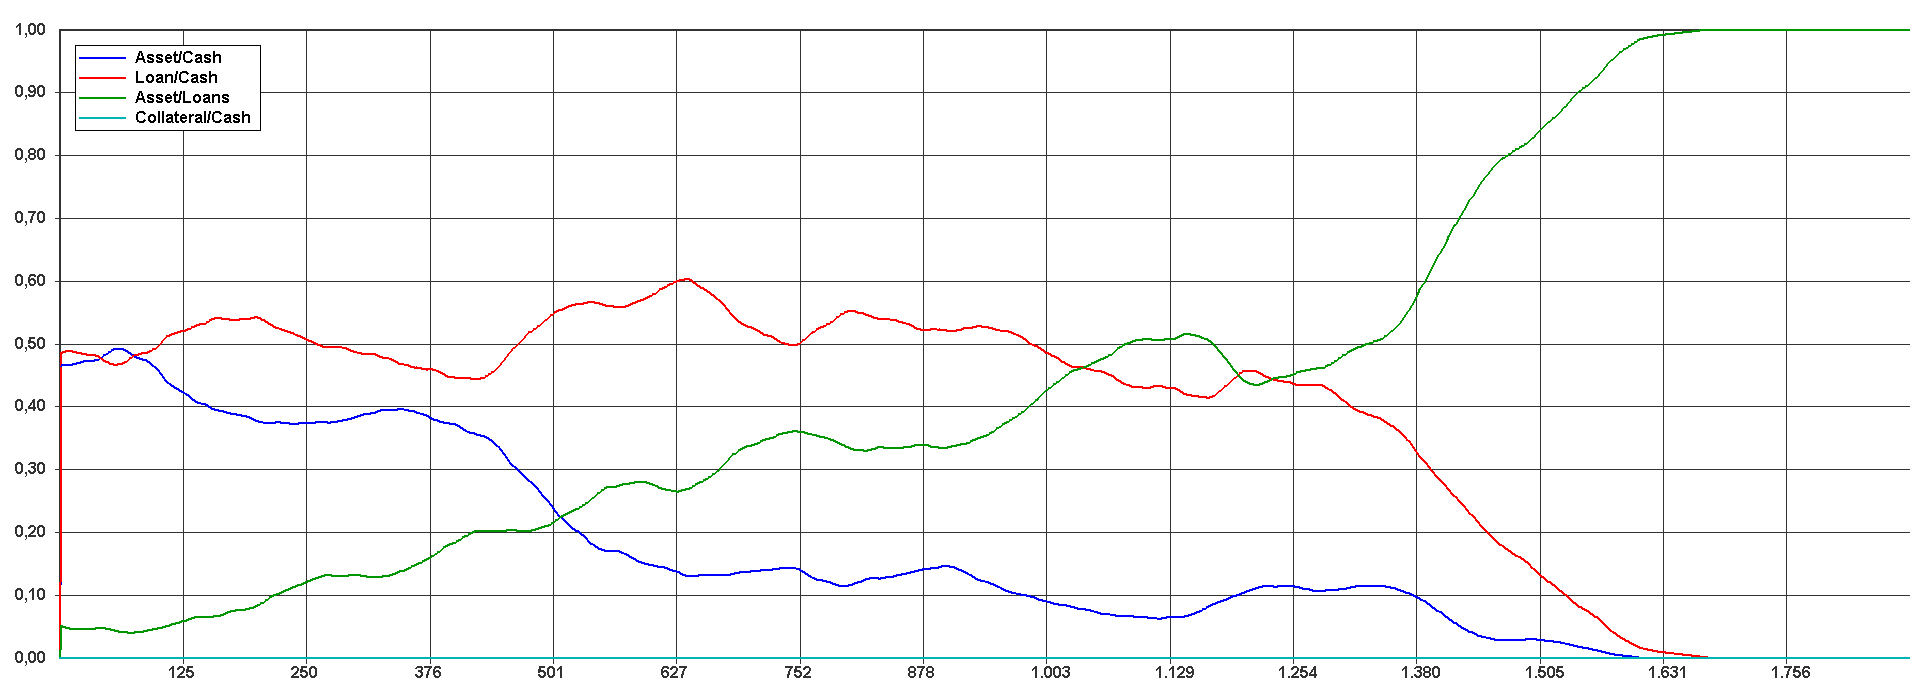
\includegraphics[width=1.0\textwidth, angle=0]{FULLYCONNECTED_100_NOCOLLATERALMARKET_MARKETSTIME_SINGLE.png}
  	\caption{Market-activity over time of Fully-Connected topology without collateral/cash market}
	\label{fig:wealth_FULLYCONNECTED_100_WITHCOLLATERALMARKET_MARKETSTIME_REPL}
\end{figure}

\begin{figure}[H]
	\centering
  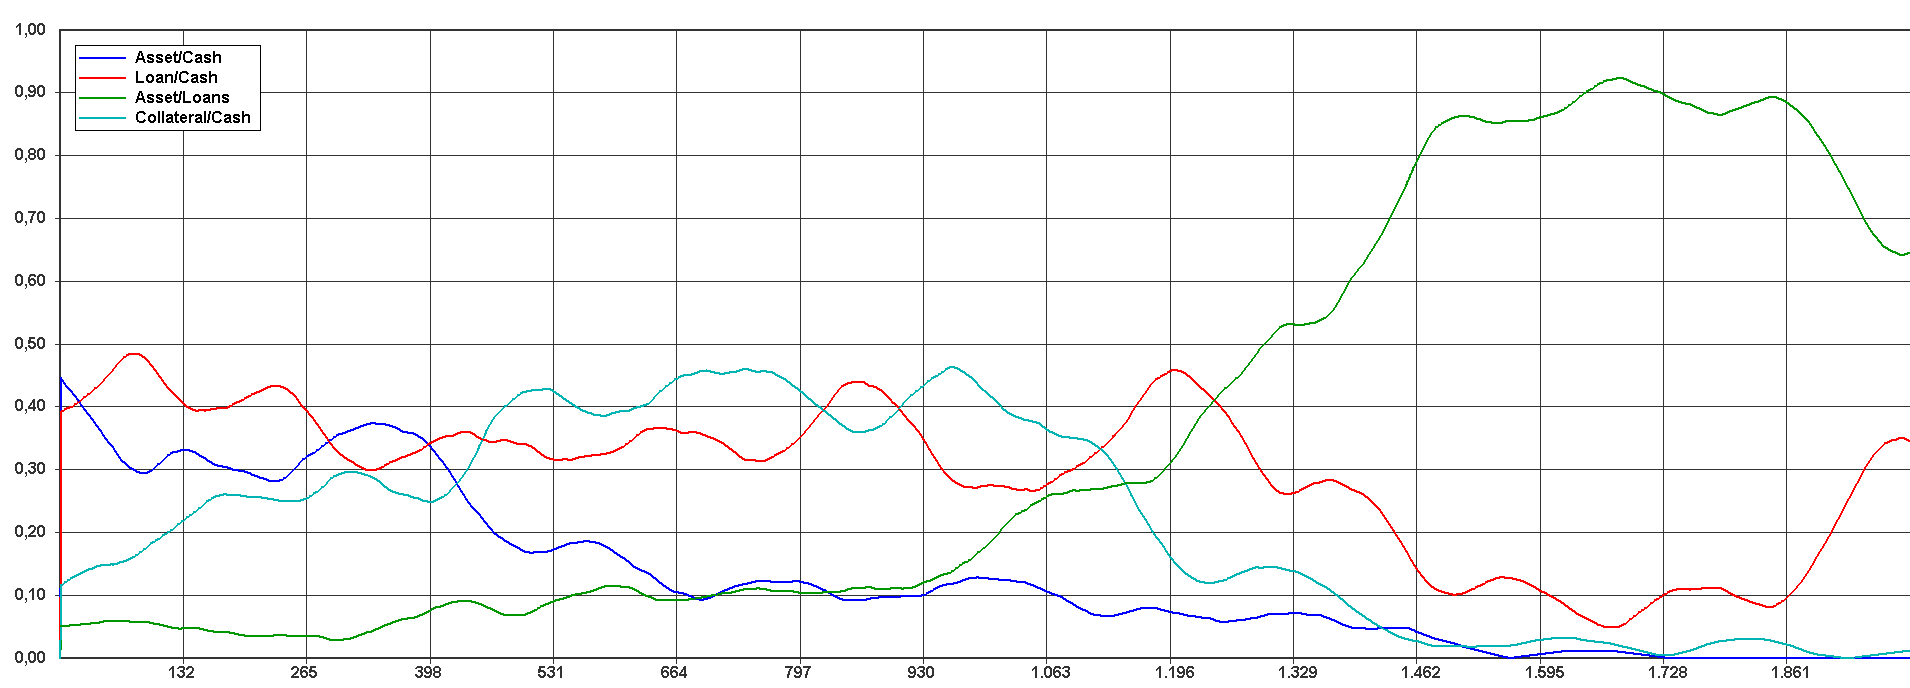
\includegraphics[width=1.0\textwidth, angle=0]{FULLYCONNECTED_100_WITHCOLLATERALMARKET_MARKETSTIME_SINGLE.png}
  	\caption{Market-activity over time of Fully-Connected topology with collateral/cash market}
	\label{fig:wealth_FULLYCONNECTED_100_WITHCOLLATERALMARKET_MARKETSTIME_REPL}
\end{figure}


\begin{figure}[H]
	\centering
  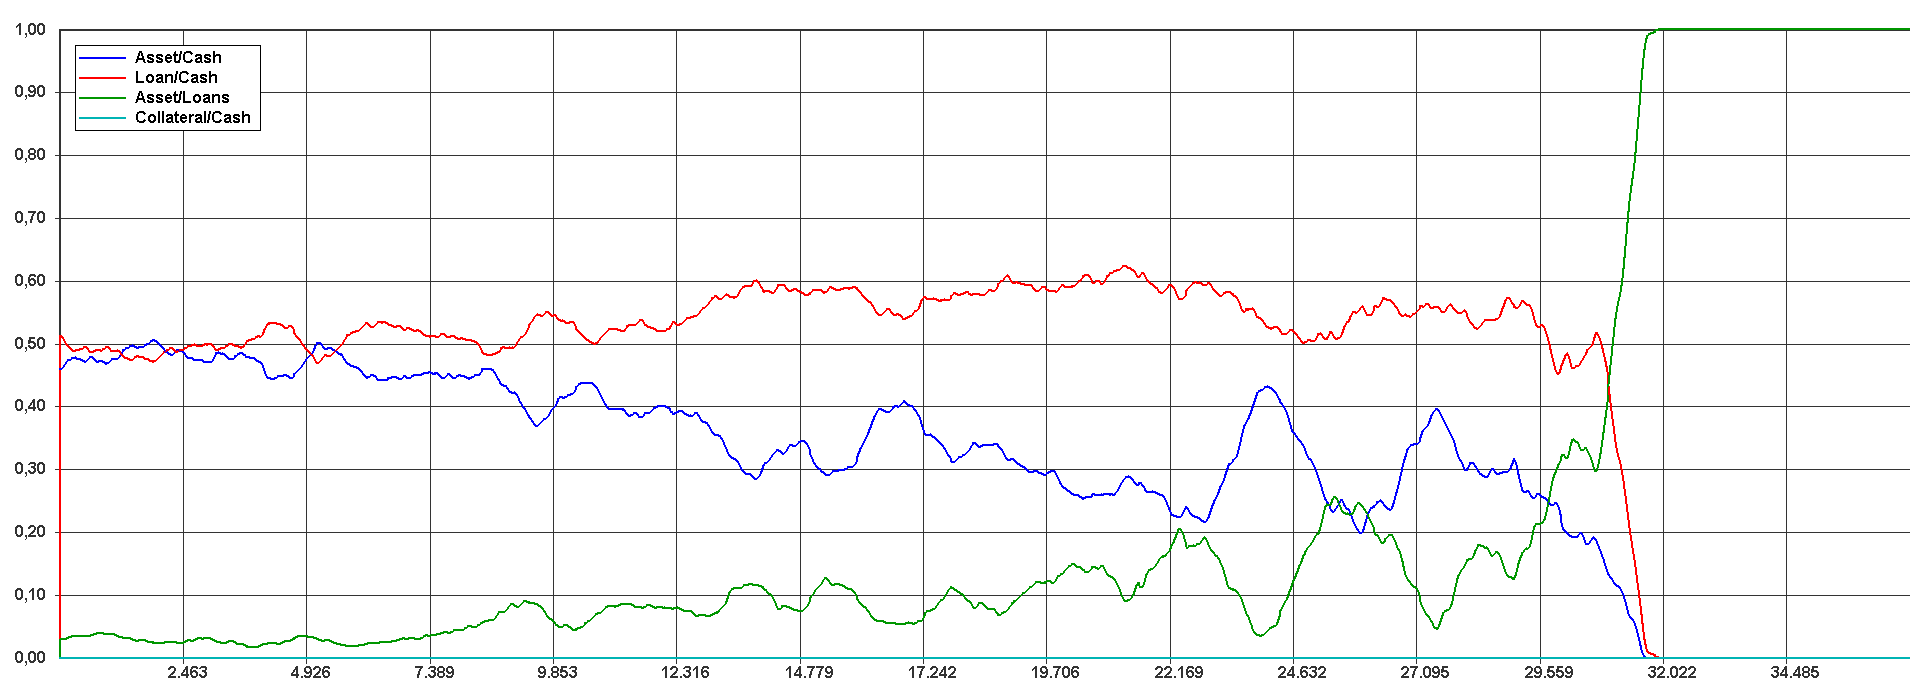
\includegraphics[width=1.0\textwidth, angle=0]{ASCENDINGCONNECTED_100_NOCOLLATERALMARKET_MARKETSTIME_SINGLE.png}
	\caption{Market-activity over time of Ascending-Connected topology without collateral/cash market}
	\label{fig:wealth_ASCENDINGCONNECTED_100_WITHCOLLATERALMARKET_MARKETSTIME_REPL}
\end{figure}

\begin{figure}[H]
	\centering
  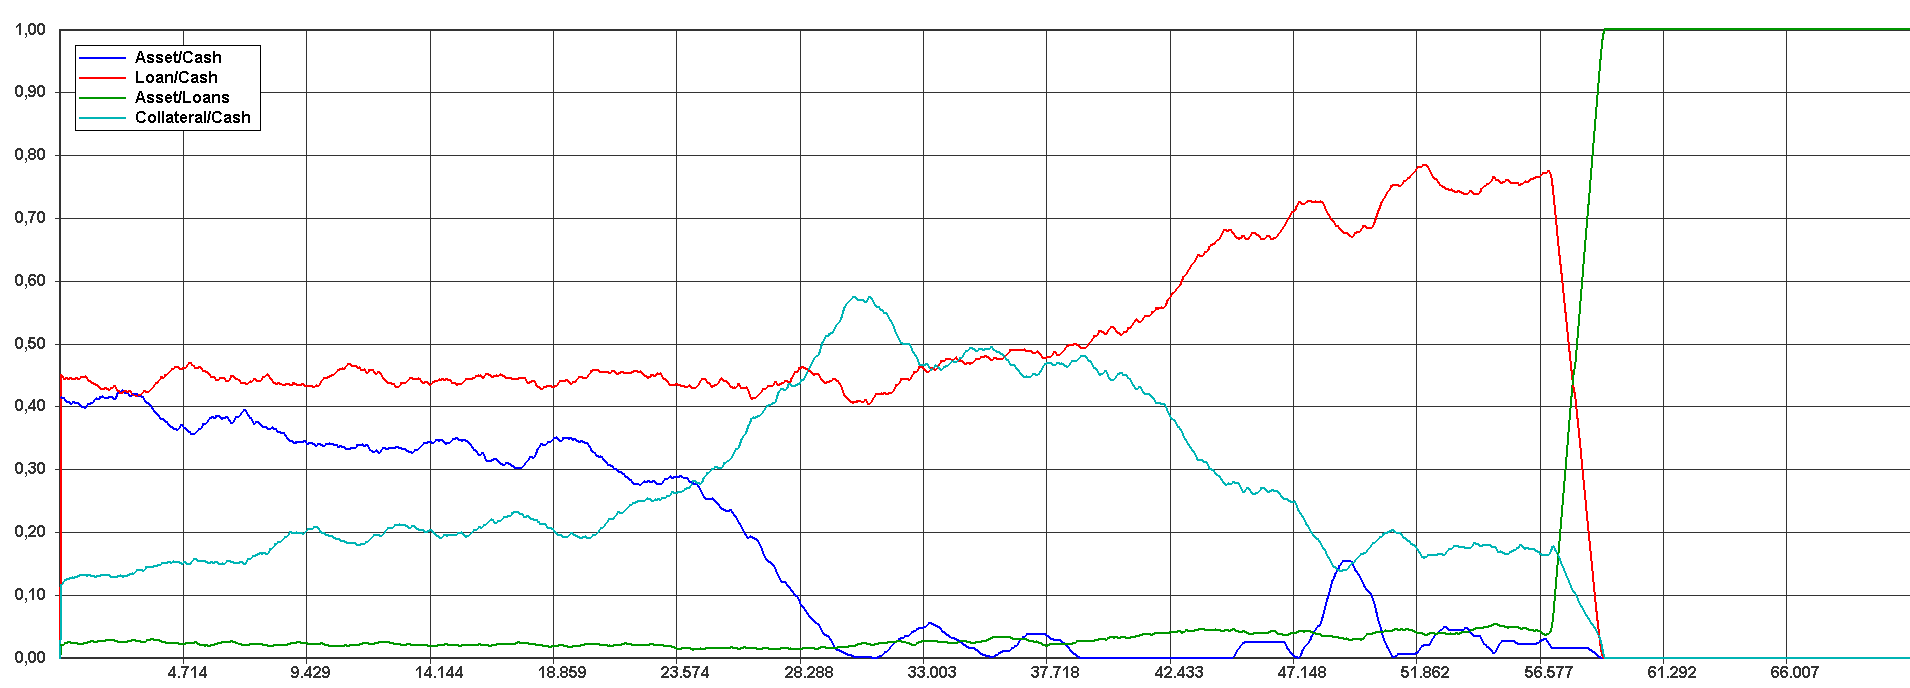
\includegraphics[width=1.0\textwidth, angle=0]{ASCENDINGCONNECTED_100_WITHCOLLATERALMARKET_MARKETSTIME_SINGLE.png}
	\caption{Market-activity over time of Ascending-Connected topology with collateral/cash market}
	\label{fig:wealth_ASCENDINGCONNECTED_100_WITHCOLLATERALMARKET_MARKETSACCUM_REPL}
\end{figure}

In the thesis-software it is possible to simulate an ascending-connected topology until no more trades are happening and then activate the new market. This feature was used to create the following figure.

\begin{figure}[H]
	\centering
  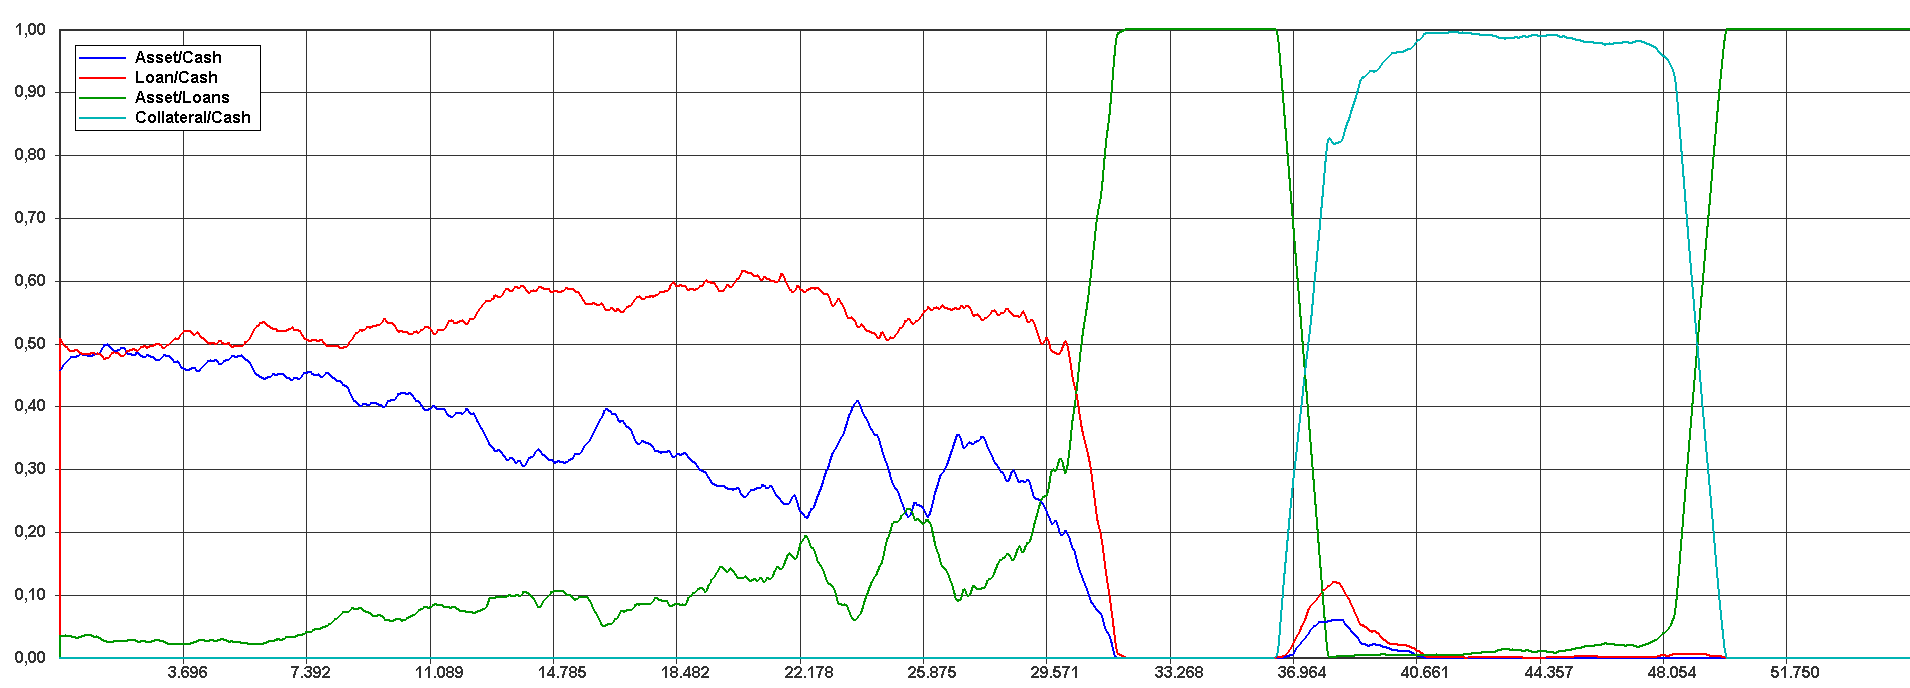
\includegraphics[width=1.0\textwidth, angle=0]{ASCENDINGCONNECTED_100_WITHCOLLATERALMARKET_DEFERREDACTIVATION_MARKETSTIME_SINGLE.png}
	\caption{Market-activity over time of Ascending-Connected topology with collateral/cash market activated after 1000 failed transactions in a row. Dynamics until activation of the new market are the same as figure \ref{fig:wealth_ASCENDINGCONNECTED_100_WITHCOLLATERALMARKET_MARKETSTIME_REPL}}
		\label{fig:wealth_ASCENDINGCONNECTED_100_WITHCOLLATERALMARKET_DEFERREDACTIVATION_MARKETSTIME_SINGLE}
\end{figure}

\section{Conclusions on new Market}
The equilibrium of the ascending-connected topology with the new market is different than the fully-connected one which reaches the theoretical equilibrium. Thus the hypothesis is still wrong because it predicted the ascending-connected topology to reach the theoretical equilibrium. This thesis can only speculate on the real reason for this but the reason is most probably rooted in the fundamental different trading dynamics in ascending-connected topology compared to fully-connected as can be seen in the market-dynamics. This thesis leaves this question open for further research.

\end{document}
